
% TODO: A plot in log-log scale that shows that your serial and parallel codes run in O(n) time and a description of the data structures that you used to achieve it. In order to get more precise timing estimates, we recommend you to run a program at least 5 times and take the median (rather than the mean) of the simulation times.
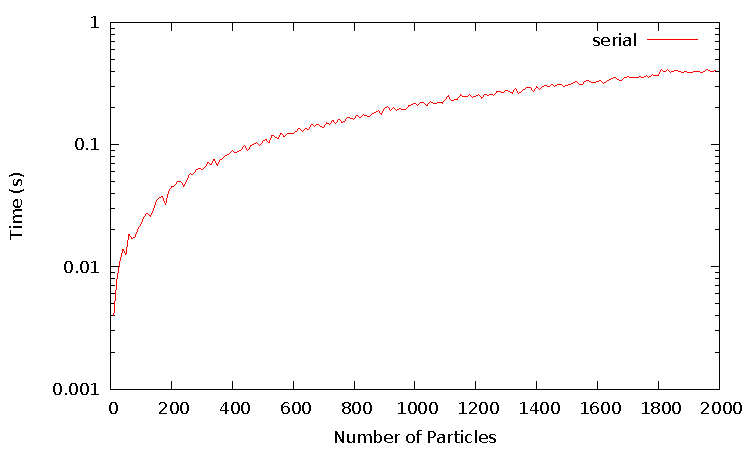
\includegraphics{plots/serial.pdf}
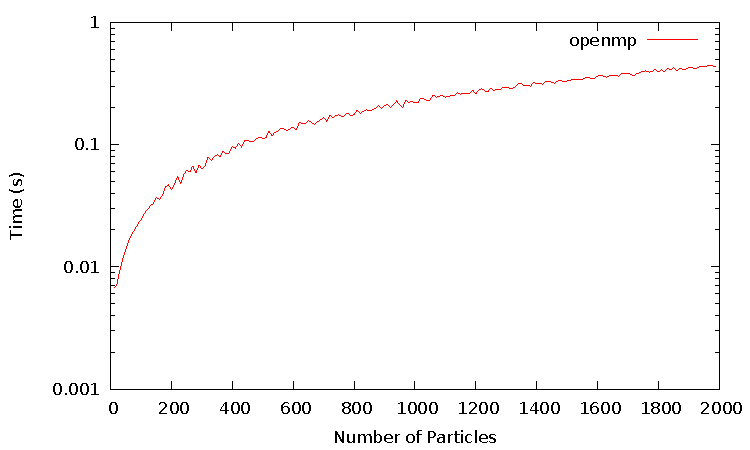
\includegraphics{plots/openmp.pdf}
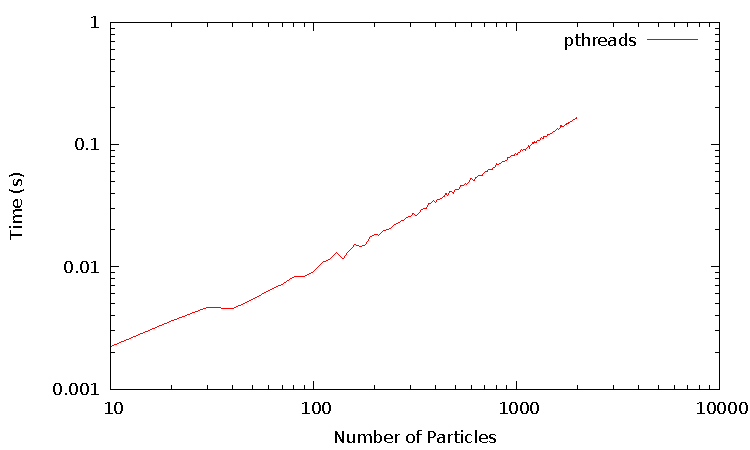
\includegraphics{plots/pthreads.pdf}

% TODO: Speedup plots that show how closely your parallel codes approach the idealized p-times speedup and a discussion on whether it is possible to do better.
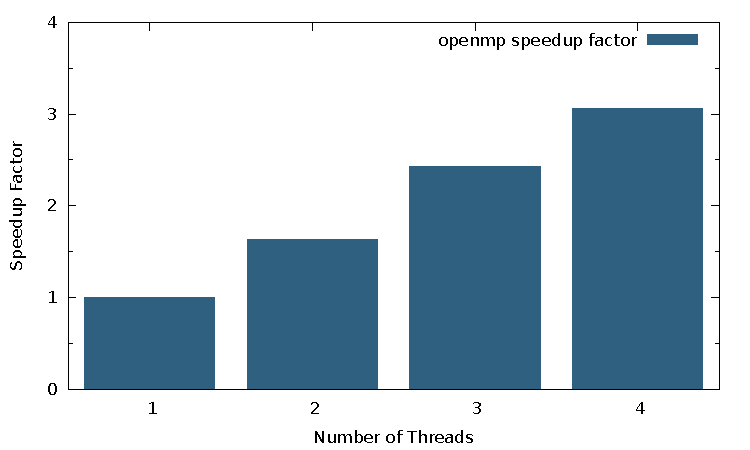
\includegraphics{plots/openmp_speedup.pdf}
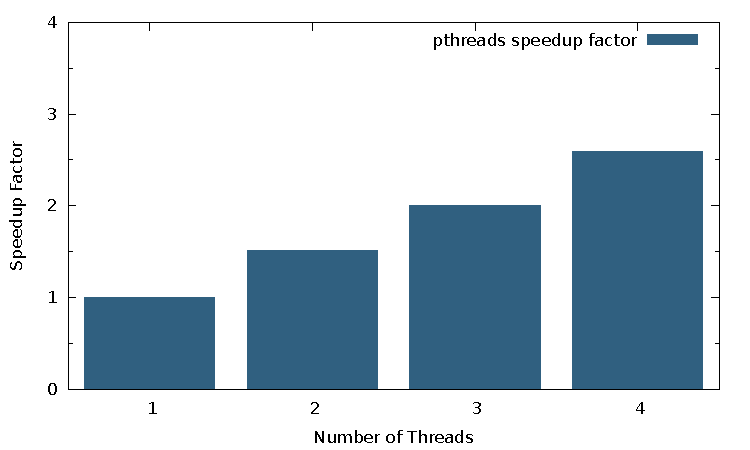
\includegraphics{plots/pthreads_speedup.pdf}

% TODO: Where does the time go? Consider breaking down the runtime into
% computation time, synchronization time and/or communication time. How do
% they scale with p?